\begin{appendices}
    
\section{K-nearest Neighbors hyperparameter optimization}\label{appendix:knn_parameters}
This figure shows the importance of different hyperparameters of the K-nearest Neighbors model regarding the R² score.


\begin{figure}[h]
    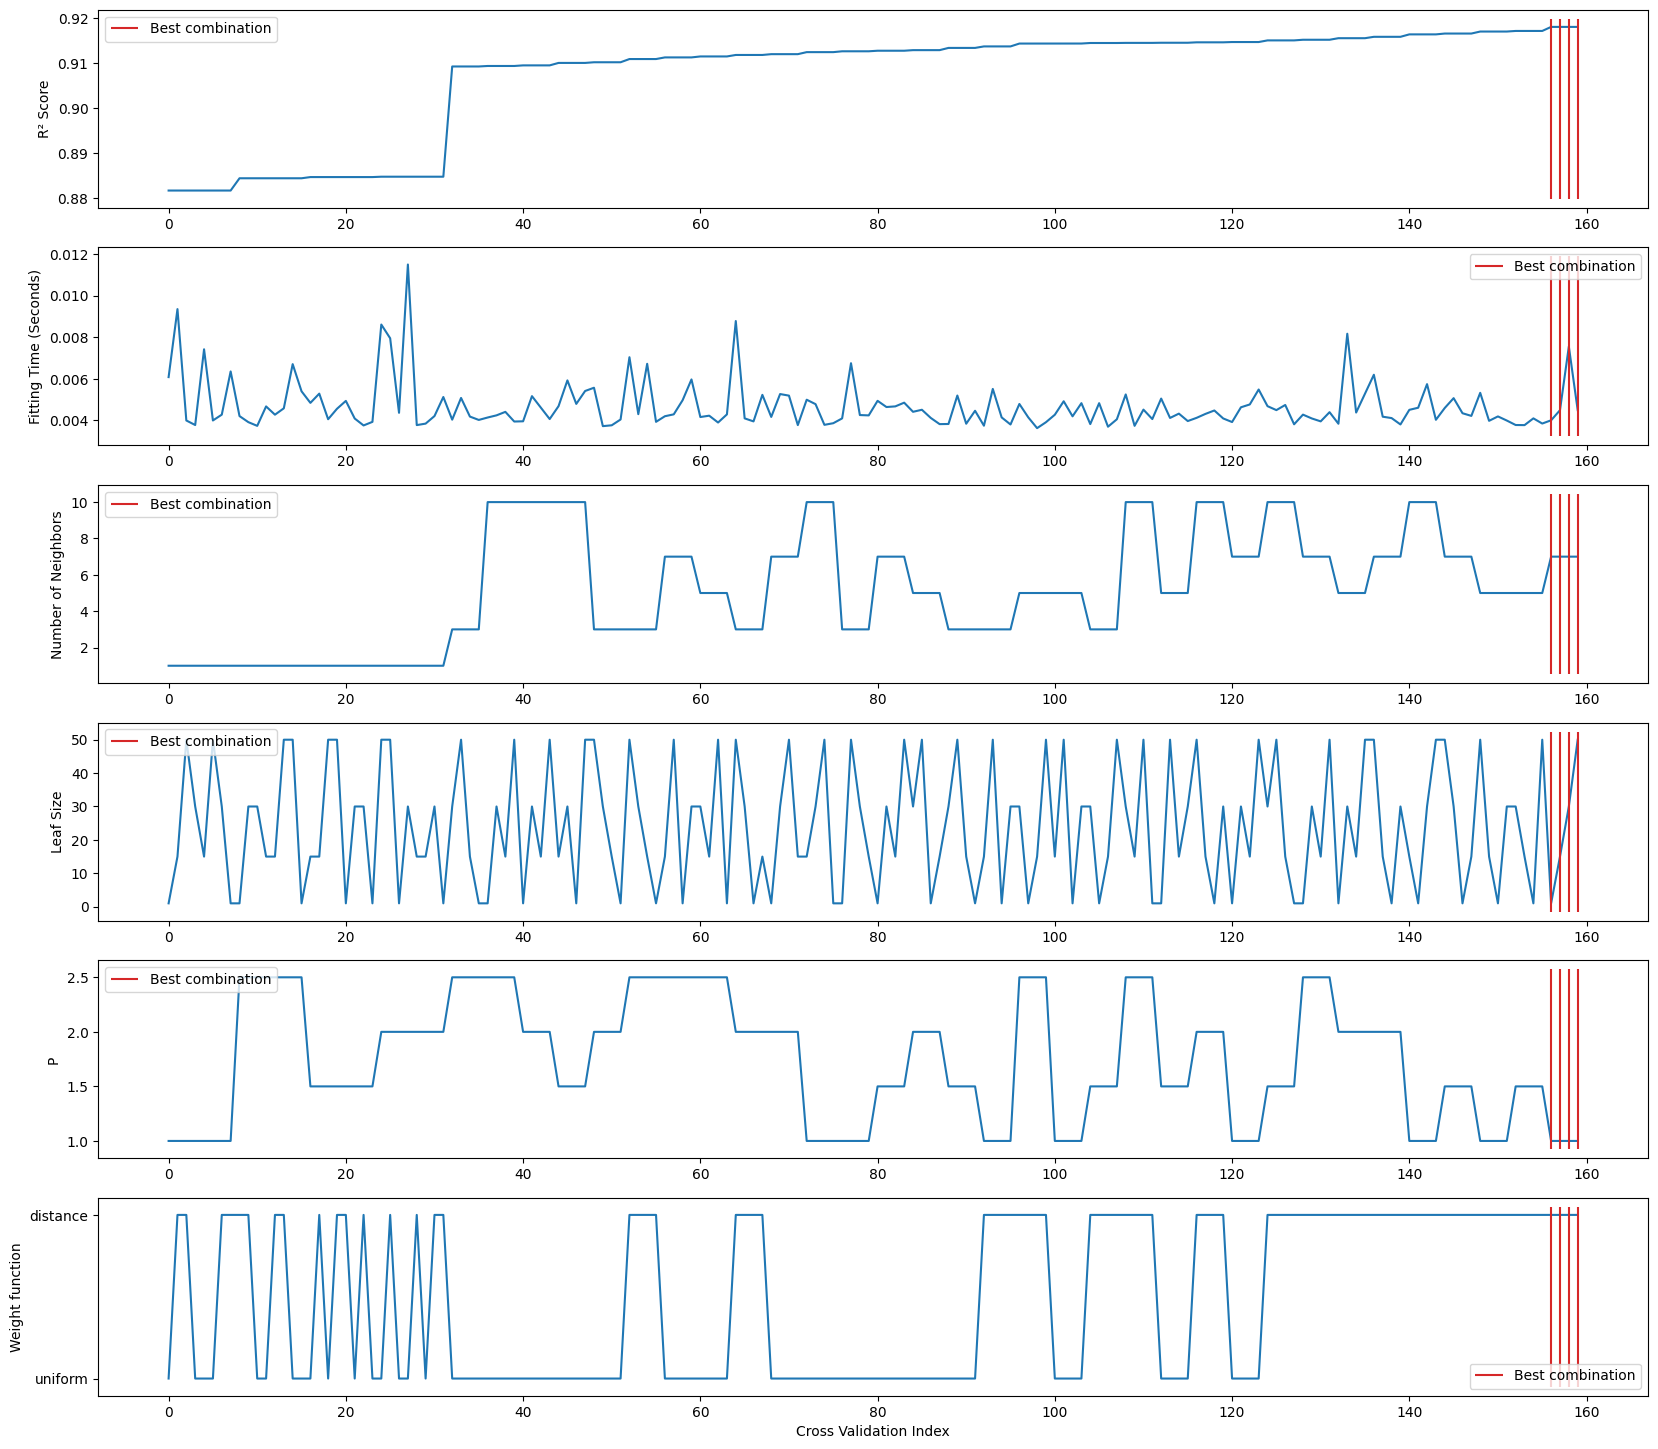
\includegraphics[width=\textwidth]{knn_hyperparameters.png}
    % \label{fig:png}
\end{figure}


\section{Distribution of Work}
We split up on the implementation and documentation between our group members, the following list shows who was mainly involved in which task:

\begin{itemize}
    \item Weather Data Cleaning: Tobias
    \item Bike Data Cleaning: Leo, Manuel
    \item Geo Data Cleaning: Laurenz, Leo, Manuel, Tobias
    \item KPI: Laurenz, Tobias
    \item Descriptive Analytics: Leo, Manuel
    \item Bike and Weather Clustering: Leo
    \item Geo Clustering: Laurenz, Leo, Manuel, Tobias
    \item Predictive Analytics: Leo, Laurenz 
    \item Report: Laurenz, Leo, Manuel, Tobias
\end{itemize}

\end{appendices}
